\section{Generative Adversarial Networks}\label{sec::gan}

A GAN consists of a generative model and a discriminative model. The objective of the generative model is to synthesize images resembling real images, while the objective of the discriminative model is to distinguish real images from synthesized ones. Both the generative and discriminative models are realized as multilayer perceptrons. 

Let $\mathbf{x}$ be a natural image drawn from a distribution, $p_{X}$, and $\mathbf{z}$ be a random vector in $\mathbb{R}^d$. Note that we only consider that $\mathbf{z}$ is from a uniform distribution with a support of $[-1\medspace\medspace 1]^d$, but different distributions such as a multivariate normal distribution can be applied as well. Let $g$ and $f$ be the generative and discriminative models, respectively. The generative model takes $\mathbf{z}$ as input and outputs an image, $g(\mathbf{z})$, that has the same support as $\mathbf{x}$. Denote the distribution of $g(\mathbf{z})$ as $p_{G}$. The discriminative model estimates the probability that an input image is drawn from $p_{X}$. Ideally, $f(\mathbf{x})=1$ if $\mathbf{x}\sim p_{X}$ and $f(\mathbf{x})=0$ if $\mathbf{x}\sim p_{G}$. The GAN framework corresponds to a minimax two-player game, and the generative and discriminative models can be trained jointly via solving 
\begin{equation}
\max_{g} \min_{f} V(f,g) \equiv E_{ \mathbf{x} \sim p_{\mathbf{X}}} [ - \log f(\mathbf{x}) ] + E_{\mathbf{z}\sim p_{\mathbf{Z}}} [ - \log( 1 - f(g(\mathbf{z}))) ].
 \label{eqn::gan_problem}
\end{equation}
In practice~(\ref{eqn::gan_problem})~is solved by alternating the following two gradient update steps:
\begin{align}
&\text{Step 1: }\medspace  \text{\boldmath$\theta$}_f^{t+1} = \text{\boldmath$\theta$}_f^{t} - \lambda^t\nabla_{\text{\boldmath$\theta$}_f} V(f^{t},g^{t}),
&\text{Step 2: }\medspace  \text{\boldmath$\theta$}_g^{t+1} = \text{\boldmath$\theta$}_g^{t} + \lambda^t\nabla_{\text{\boldmath$\theta$}_g} V(f^{t+1},g^{t})\nonumber
\end{align}
where $\text{\boldmath$\theta$}_f$ and $\text{\boldmath$\theta$}_g$ are the parameters of $f$ and $g$, $\lambda$ is the learning rate, and $t$ is the iteration number. %of the gradient updates. 

Goodfellow et al.~\cite{goodfellow2014generative} show that, given enough capacity to $f$ and $g$ and sufficient training iterations, the distribution, $p_{G}$, converges to $p_{X}$. In other words, from a random vector, $\mathbf{z}$, the network $g$ can synthesize an image, $g(\mathbf{z})$, that resembles one that is drawn from the true distribution, $p_X$.

\section{Coupled Generative Adversarial Networks}\label{sec::dgan}

CoGAN as illustrated in Figure~\ref{fig::DGAN} is designed for learning a joint distribution of images in two different domains. It consists of a pair of GANs---$\text{GAN}_1$ and $\text{GAN}_2$; each is responsible for synthesizing images in one domain. During training, we force them to share a subset of parameters. This results in that the GANs learn to synthesize pairs of corresponding images without correspondence supervision. 

{\bf Generative Models: }
Let $\mathbf{x}_1$ and $\mathbf{x}_2$ be images drawn from the marginal distribution of the 1st domain, $\mathbf{x}_1\sim p_{X_1}$ and the marginal distribution of the 2nd domain, $\mathbf{x}_2\sim p_{X_2}$, respectively. Let $g_1$ and $g_2$ be the generative models of $\text{GAN}_1$ and $\text{GAN}_2$, which map a random vector input $\mathbf{z}$ to images that have the same support as $\mathbf{x}_1$ and $\mathbf{x}_2$, respectively. Denote the distributions of $g_1(\mathbf{z})$ and $g_1(\mathbf{z})$ by $p_{G_1}$ and $p_{G_2}$. Both $g_1$ and $g_2$ are realized as multilayer perceptrons: 
\begin{align}
& g_1(\mathbf{z}) = g_1^{(m_1)}\big{(}g_1^{(m_1-1)}\big{(}\ldots\medspace g_1^{(2)}\big{(}g_1^{(1)}(\mathbf{z})\big{)}\big{)}\big{)},\quad
g_2(\mathbf{z}) = g_2^{(m_2)}\big{(}g_2^{(m_2-1)}\big{(}\ldots\medspace g_2^{(2)}\big{(}g_2^{(1)}(\mathbf{z})\big{)}\big{)}\big{)}\nonumber
\end{align}
where $g_1^{(i)}$ and $g_2^{(i)}$ are the $i$th layers of $g_1$ and $g_2$ and $m_1$ and $m_2$ are the numbers of layers in $g_1$ and $g_2$. Note that $m_1$ need not equal $m_2$. Also note that the support of $\mathbf{x}_1$ need not equal to that of $\mathbf{x}_2$.

Through layers of perceptron operations, the generative models gradually decode information from more abstract concepts to more material details. The first layers decode high-level semantics and the last layers decode low-level details. Note that this information flow direction is opposite to that in a discriminative deep neural network~\cite{krizhevsky2012imagenet} where the first layers extract low-level features while the last layers extract high-level features. 

Based on the idea that a pair of corresponding images in two domains share the same high-level concepts, we force the first layers of $g_1$ and $g_2$ to have identical structure and share the weights. That is 
$\text{\boldmath$\theta$}_{g_1^{(i)}}=\text{\boldmath$\theta$}_{g_2^{(i)}}, \text{for } i=1,2,...,k$
where $k$ is the number of shared layers, and $\text{\boldmath$\theta$}_{g_1^{(i)}}$ and $\text{\boldmath$\theta$}_{g_2^{(i)}}$ are the parameters of $g_1^{(i)}$ and $g_2^{(i)}$, respectively. This constraint forces the high-level semantics to be decoded in the same way in $g_1$ and $g_2$. No constraints are enforced to the last layers. They can materialize the shared high-level representation differently for fooling the respective discriminators.

\begin{figure}[t!]
\centering
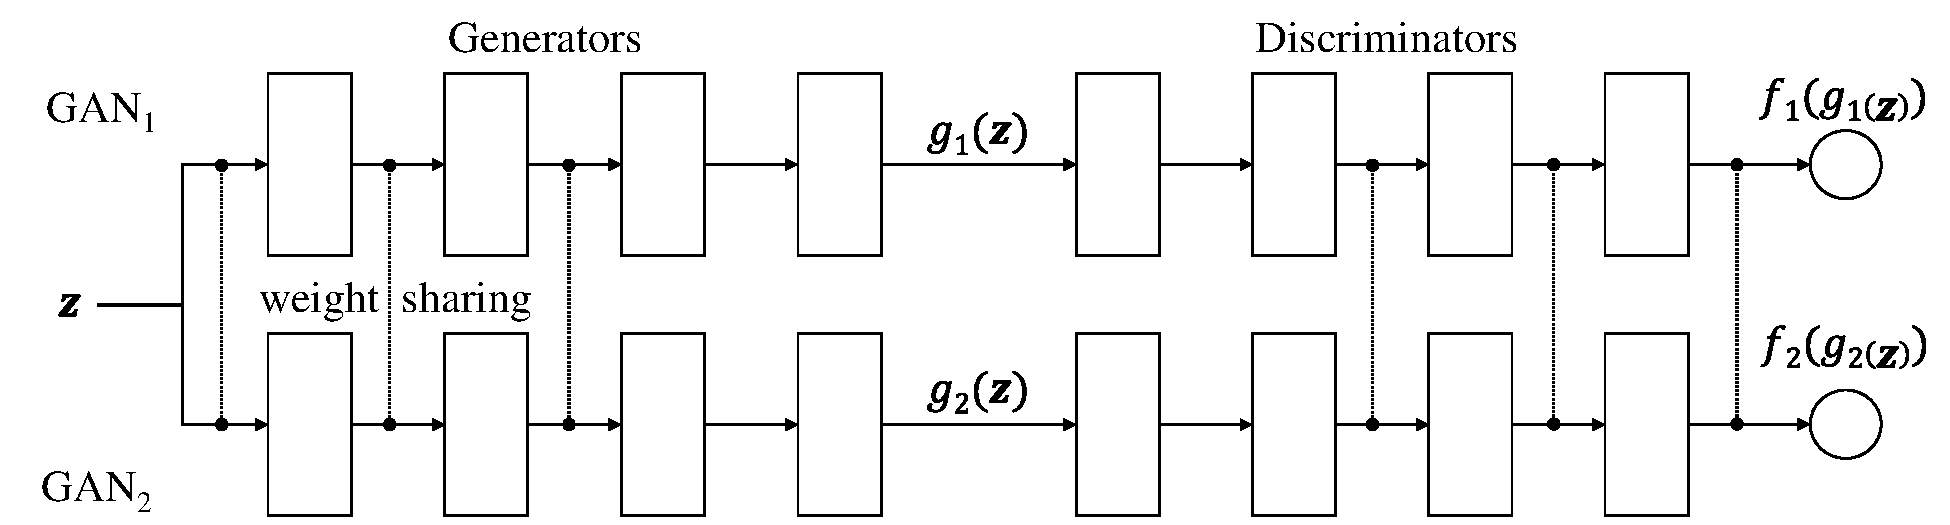
\includegraphics[trim=0.05in 0.1in 0.05in 0.2in,width=.96\linewidth]{overview_landscape_very_tight.pdf}
\caption{\small CoGAN consists of a pair of GANs: $\text{GAN}_1$ and $\text{GAN}_2$. Each has a generative model for synthesizing realistic images in one domain and a discriminative model for classifying whether an image is real or synthesized. We tie the weights of the first few layers (responsible for decoding high-level semantics) of the generative models, $g_1$ and $g_2$. We also tie the weights of the last few layers (responsible for encoding high-level semantics) of the discriminative models, $f_1$ and $f_2$. This weight-sharing constraint allows CoGAN to learn a joint distribution of images without correspondence supervision. A trained CoGAN can be used to synthesize pairs of corresponding images---pairs of images sharing the same high-level abstraction but having different low-level realizations.}
\label{fig::DGAN}
\end{figure}

{\bf Discriminative Models: }
Let $f_1$ and $f_2$ be the discriminative models of $\text{GAN}_1$ and $\text{GAN}_2$ given by
\begin{align}
& f_1(\mathbf{x}_1) = f_1^{(n_1)}\big{(}f_1^{(n_1-1)}\big{(}\ldots\medspace f_1^{(2)}\big{(}f_1^{(1)}(\mathbf{x}_1)\big{)}\big{)}\big{)},\medspace
f_2(\mathbf{x}_2) = f_2^{(n_2)}\big{(}f_2^{(n_2-1)}\big{(}\ldots\medspace f_2^{(2)}\big{(}f_2^{(1)}(\mathbf{x}_2)\big{)}\big{)}\big{)}\nonumber
\end{align}
where $f_1^{(i)}$ and $f_2^{(i)}$ are the $i$th layers of $f_1$ and $f_2$ and $n_1$ and $n_2$ are the numbers of layers. The discriminative models map an input image to a probability score, estimating the likelihood that the input is drawn from a true data distribution. The first layers of the discriminative models extract low-level features, while the last layers extract high-level features. Because the input images are realizations of the same high-level semantics in two different domains, we force $f_1$ and $f_2$ to have the same last layers, which is achieved by sharing the weights of the last layers via
$\text{\boldmath$\theta$}_{f_1^{(n_1-i)}}=\text{\boldmath$\theta$}_{f_2^{(n_2-i)}}, \text{for } i=0,1,...,l-1$
where $l$ is the number of weight-sharing layers in the discriminative models, and $\text{\boldmath$\theta$}_{f_1^{(i)}}$ and $\text{\boldmath$\theta$}_{f_2^{(i)}}$ are the network parameters of $f_1^{(i)}$ and $f_2^{(i)}$, respectively. The weight-sharing constraint in the discriminators helps reduce the total number of parameters in the network, but it is not essential for learning a joint distribution.

{\bf Learning: }
The CoGAN framework corresponds to a constrained minimax game given by
\begin{align}
 \max_{g_1,g_2} \min_{f_1,f_2} \medspace V(f_1,f_2,g_1,g_2), \medspace \text{ subject to }\quad 
&\text{\boldmath$\theta$}_{g_1^{(i)}}=\text{\boldmath$\theta$}_{g_2^{(i)}}, \quad\quad\quad\text{for $i=1,2,...,k$} \quad \\
&\text{\boldmath$\theta$}_{f_1^{(n_1-j)}}=\text{\boldmath$\theta$}_{f_2^{(n_2-j)}}, \space\space\text{ for $j=0,1,...,l-1$} \nonumber
\end{align}
where the value function $V$ is given by 
\begin{align}
V(f_1,f_2,g_1,g_2) &= E_{ \mathbf{x}_1 \sim p_{\mathbf{X}_1}} [ - \log f_1(\mathbf{x}_1) ] + E_{\mathbf{z}\sim p_{\mathbf{Z}}} [ - \log( 1 - f_1(g_1(\mathbf{z}))) ]\nonumber\\
& + E_{ \mathbf{x}_2 \sim p_{\mathbf{X}_2}} [ - \log f_2(\mathbf{x}_2) ]+ E_{\mathbf{z}\sim p_{\mathbf{Z}}} [ - \log( 1 - f_2(g_2(\mathbf{z}))) ].
\end{align}
In the game, there are two teams and each team has two players. The generative models form a team and work together for synthesizing a pair of images in two different domains for confusing the discriminative models. The discriminative models try to differentiate images drawn from the training data distribution in the respective domains from those drawn from the respective generative models. The collaboration between the players in the same team is established from the weight-sharing constraint. Similar to GAN, CoGAN can be trained by back propagation with the alternating gradient update steps. The details of the learning algorithm are given in the supplementary materials.

{\bf Remarks:} CoGAN learning requires training samples drawn from the marginal distributions, $p_{X_1}$ and $p_{X_2}$. It does not rely on samples drawn from the joint distribution, $p_{X_1,X_2}$, where corresponding supervision would be available. Our main contribution is in showing that with just samples drawn separately from the marginal distributions, CoGAN can learn a joint distribution of images in the two domains. Both weight-sharing constraint and adversarial training are essential for enabling this capability. Unlike autoencoder learning~\cite{ngiam2011multimodal}, which encourages a generated pair of images to be {\it identical} to the target pair of corresponding images in the two domains for minimizing the reconstruction loss\footnote{This is why \cite{ngiam2011multimodal} requires samples from the joint distribution for learning the joint distribution.}, the adversarial training only encourages the generated pair of images to be {\it individually resembling to} the images in the respective domains. With this more relaxed adversarial training setting, the weight-sharing constraint can then kick in for capturing correspondences between domains. With the weight-sharing constraint, the generative models must utilize the capacity more efficiently for fooling the discriminative models, and the most efficient way of utilizing the capacity for generating a pair of realistic images in two domains is to generate a pair of {\it corresponding} images since the neurons responsible for decoding high-level semantics can be shared. 

CoGAN learning is based on existence of shared high-level representations in the domains. If such a representation does not exist for the set of domains of interest, it would fail.
